\section{PLL: Phase Locked-Loop}

\subsection{Introducci\'on}

Un Phase Locked-Loop, mejor conocido como PLL, es un sistema de control cuya se\~nal de salida tiene la misma frecuencia que la se\~nal de entrada y sigue sus variaciones en frecuencia dentro de un rango acotado. El PLL es muy usado en sistemas de comunicaciones, ya que sus principales aplicaciones son de demodulador de FM o PM y como seguidor o sincronizador de se\~nales que temporalmente var\'ian su frecuencia. A continuaci\'on se analizar\'an ciertos comportamientos del PLL y su aplicaci\'on como demodulador de FM y como multiplicador de frecuencia. Para realizar el trabajo se utilizar\'a el integrado CD4046 \footnote{Hoja de datos del integrado CD4046:}.
\todo{agregar datasheet}

\subsection{Diagrama en bloques del PLL}

El PLL est\'a formado por tres bloques fundamentales para su funcionamiento: un comparador de fase, un filtro pasabajos y un oscilador controlado por tensi\'on (mejor conocido como VCO y que ser\'a estudiado en profundidad en la \'ultima secci\'on). Esta distribuci\'on en bloques es mostrada en la figura \ref{pll}.

\begin{figure}[H] %!ht
	\centering
	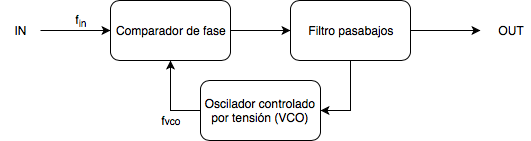
\includegraphics[width=12cm,height=12cm,keepaspectratio]{../EJ2/imagenes/PLL.png}
	\caption{Diagrama en bloques del PLL.}
	\label{pll}
\end{figure}

	\subsubsection{Comparador de fase}
	Del comparador de fase sale una tensi\'on proporcional a la diferencia de fase entre la se\~nal de entrada y aquella que proviene del VCO. Llamando a la tensi\'on de salida del comparador $V_1$, a la ganancia del valor de fase $K_{\phi}$ (la expresi\'on que la determina depende de la forma de implementar el comparador)y a la diferencia de fase entre la se\~nal de entrada y la proveniente del VCO $\Delta_{phi}$:
	
	\begin{equation}
		\begin{cases}
			V_1 = K_{\phi} \cdot \Delta_{\phi} \\
			\Delta_{\phi} = \phi_{in} - \phi_{vco} = \frac{\Delta t}{T}\cdot 2 \pi 	
		\end{cases}
	\end{equation}
	
	Se mencion\'o que hay distintas formas de implementar un comparador. El integrado que se emplea en este trabajo es el CD4046 y contiene dos tipos de comparadores de fase diferentes (tipo 1 y tipo 2) 
	\todo{explicar los comparadores del integrado usado}
	
	\subsubsection{Filtro pasabajos}
	Este filtro se emplea para que el lazo sea estable. Tambi\'en permite un proceso de captura de frecuencias m\'as rapido, un rango de captura mayor y la respuesta del circuito no es sobre amortiguada. Adem\'as, en caso de que se pierda el enganche por interferencias durante el transitorio, el filtro otorga una memoria en el lazo. Por otro lado, la presencia del filtro brinda una ventaja en la demodulaci\'on. La señal que sale del comparador de fase ingresar\'a luego al VCO. Si esta señal tiene un riple, al demodularla puede producir picos no correspondientes a la señal que inicialmente fue modulada.
		
	\subsubsection{VCO: Voltage Controlled Oscillator}
	El VCO es un integrador que genera una señal cuya frecuencia es proporcional a la tensi\'on de la señal aplicada en su entrada:
	
	\begin{equation}
		\begin{cases}
			\omega_{vco} =\omega_0 + K_{vco} \cdot V_2\\
			\omega_{vco} = \frac{d \phi_{vco}}{dt} \implies \phi_{vco} = \int \omega_{vco} dt \implies \phi_{vco}(s) = \frac{1}{s} \cdot \omega_{vco}(s)
		\end{cases}
	\end{equation}
	
	Siendo, en las ecuaciones anteriores, $\omega_{vco}$ la frecuencia a la salida del VCO, $\omega_0$ la frecuencia de la señal que entra al VCO, denominada "free running frequency" y $K_{vco}$ la constante de proporcionalidad que introduce el VCO.
	
	
\subsection{Respuesta en frecuencia}

Se respresenta ahora el diagrama en bloques indicando matem\'aticamente la influencia de cada uno, para mostrar a partir de este la funci\'on transferencia del PLL.

\begin{figure}[H] %!ht
	\centering
	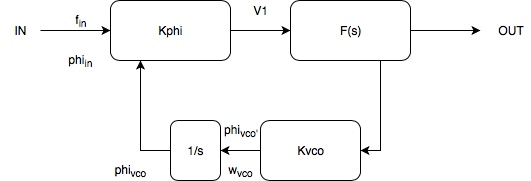
\includegraphics[width=12cm,height=12cm,keepaspectratio]{../EJ2/imagenes/transf.png}
	\caption{Diagrama en bloques del PLL con sus funciones matem\'aticas.}
	\label{pll2}
\end{figure}

A partir del diagrama en bloques de la figura \ref{pll2}, se hace el siguiente desarrollo matem\'atico. Se parte de:
\begin{equation}
	\begin{cases}
		H(s) = \frac{G(s)}{1+G(s)}\\
		G(s) = \frac{K_{\phi}F(s)K_{vco}}{s}
	\end{cases}
\end{equation}

Luego, 

\begin{equation}
\begin{cases}
	\frac{V_{out}}{\phi_{in}} = \frac{sK_{\phi}F(s)}{s+K_{\phi}K_{vco}F(s)}\\ \\
	\frac{V_{out}}{\omega_{in}}=\frac{V_{out}}{\phi_{in}s} = \frac{K_{\phi}F(s)}{s+K_{\phi}K_{vco}F(s)}
	\end{cases}
	\label{transf}
\end{equation}

Y entonces se puede escribir $G(s)$ como:

\begin{equation}
	G(s) = \frac{K_{vco}F(s)}{s}
\end{equation}
	
Adem\'as:

\begin{equation}
	\phi_{vco} = \frac{G(s)}{1+G(s)}\phi_{in}(s)
\end{equation}

Y por el teorema del valor final, sabemos que $\lim_{t\rightarrow\infty}{x(t)} = \lim_{s\rightarrow0}{sX(s)}$:

\begin{equation}
	\lim_{s\rightarrow0}{s\phi_{vco}(s)} = \lim_{s\rightarrow0}{s\left( \frac{G(s)}{1 + G(s)}\phi_{in}(s) \right)} = \phi_{in} (s)
\end{equation}

Por lo tanto:

\begin{equation}
	\phi_{vco}(t) \approx \phi_{in}(t)|_{t\to\infty} 
	\label{futuro}
\end{equation}

La interpretaci\'on del resultado en la ecuaci\'on \ref{futuro} es que una vez alcanzado el comportamiento permanente del circuito, la fase de la señal de salida del VCO sigue a aquella de la señal de entrada y a esto se debe lo mencionado al inicio sobre que estas señales presentan la misma frecuencia.

	\subsubsection{Transferencia en condici\'on de enganche}

\subsection{Respuesta al escal\'on}
	En el caso del PLL, se ha observado que estudiar la funci\'on transferencia del circuito consiste en analizar qu\'e sucede con la tensi\'on de salida en funci\'on de la frecuencia de entrada. Debido a esto, estudiar la respuesta al escal\'on es ver el comportamiento de la tensi\'on de salida a partir de un "escal\'on en frecuencia". Es decir, el escal\'on es un cambio abrupto entre señales con dos frecuencias separadas por un intervalo de valores. Es importante remarcar que ambas frecuencias deben estar dentro del rango de captura por que de lo contrario no podr\'ian engancharse y la respuesta a este cambio de frecuencias no podr\'ia ser medida. Para medir esto, se configur\'o una señal en el generador de señales a una frecuencia dada. Luego se modific\'o el valor de la frecuencia utilizando los botones del instrumento ya que se deseaba obtener un cambio brusco de frecuencias, y se emple\'o el osciloscopio en modo Single para poder ver la respuesta del circuito frente a este cambio.

	\subsubsection{Factor de calidad a partir del overshoot}

	\subsubsection{Tiempo de establecimiento}

\subsection{Rango de captura y de enganche}

\begin{figure}[H] %!ht
	\centering
	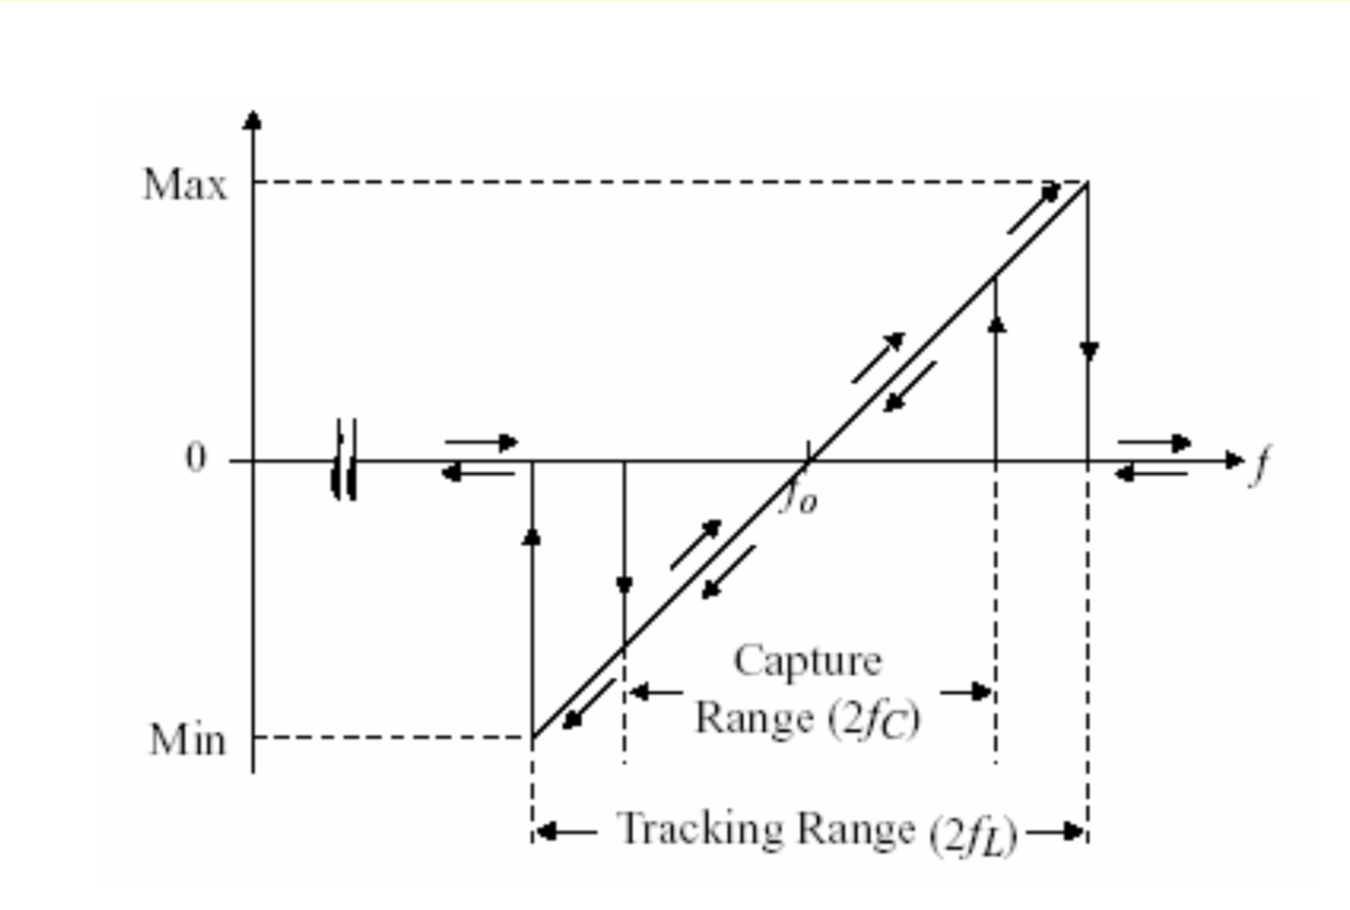
\includegraphics[width=12cm,height=12cm,keepaspectratio]{../EJ2/imagenes/rango.png}
	\caption{Rangos de captura y de enganche.}
	\label{rango}
\end{figure}

	\paragraph{Rango de captura:} Es el rango de frecuencias en el que la señal de entrada debe estar para para engancharse. El rango de captura es $2f_c$, siendo $f_c$ la frecuencia de captura, medida desde una frecuencia central $f_0$. Esto se ve en la figura \ref{rango}.

	\paragraph{Rango de enganche:} Es el rango de frecuencias para el cual la señal a la salida del VCO queda enganchada luego de haver pasado por el rango de captura. El rango de enganche es $2f_L$, siendo $f_L$ la freciencia de enganche, medida respecto a la frecuencia $f_0$. Esto se ve en la figura \ref{rango}.
	
	El rango de captura es menor al rango de enganche, ya que para quedar enganchada la señal luego de pasar por el VCO, debe haber pasado previamente por el rango de captura. Por lo tanto $2f_C<2f_L$.

\subsection{Respuesta transitoria ante distintos filtros de lazo}

	\subsubsection{Sin filtro: F(s) = 1 }
	Haciendo $F(s) = 1$ en la expresi\'on \ref{transf}, se obtiene:
	
\begin{equation}
\begin{cases}
\frac{V_{out}}{\phi_{in}} = \frac{sK_{\phi}}{s+K_{\phi}K_{vco}}\\ \\
\frac{V_{out}}{\omega_{in}}=\frac{V_{out}}{\phi_{in}s} = \frac{K_{\phi}}{s+K_{\phi}K_{vco}}
\end{cases}
\label{transf1}
\end{equation}

Considerando la segunda espresi\'on de \ref{transf1}, se observa que es de la forma de un filtro pasabajos. La variable de entrada es$\omega_{in}$. La respuesta de esta expresi\'on representa una tensi\'on que corresponde a haber modulado en frecuencia una onda portadora entrante.
Se mencionan ciertas caracter\'isticas del comportamiento del circuito sin la presencia del filtro F(s). Dado que del comparador sale una señal con una frecuencia de la suma de las de sus entradas y otra con la resta, no habr\'a un filtro luego del comparador que permita el paso de solo una de ellas. Tambi\'en pueden aparecer señales de interferencia no pertenicientes a la banda deseada. El PLL con este tipo de filtro tiene un proceso de captura m\'as lento, un menor rango de captura y una respuesta sobre amortiguada. Sin embargo, rechaza m\'as aquellas perturbaciones en la frecuencia que entra.
Por otro lado, el VCO genera una señal cuya frecuencia var\'ia en funci\'on de un valor de tensi\'on cont\'inua a su entrada. Sin la presencia de ning\'un filtro a la entrada del VCO, al mismo le llega una señal que no es cont\'inua, ya que proviene directamente de la salida del comparador. Sin embargo, el VCO debe recibir tensi\'on cont\'inua a su entrada para funcionar correctamente. Si la tensi\'on a su entrada no es cont\'inua, el VCO deber\'a tratar de seguir a la señal que le llega. Debido a que su respuesta no es instant\'anea, no logra seguir su tensi\'on de un lado a otro y por lo tanto esto resulta en que el VCO responde a una señal pr\'acticamente plana, variando su valor cercanamente al valor medio de su señal de entrada. Lo que en realidad deber\'a suceder es que a la entrada del VCO llegue una tensi\'on cont\'inua. Esto puede lograrse colocando un integrador antes del VCO de forma que la señal de entrada al mismo sea el valor medio (un valor de tensi\'on constante) de la señal de salida del comparador. Para lograrlo, se agrega un filtro F(s), como los mencionados a continuaci\'on.
		
	\subsubsection{Filtro pasa bajos: RC}
	
	Teniendo un filtro pasa bajos de la forma $F(s) = \frac{1}{\frac{s}{\omega_p} + 1}$, reemplazando esto en la expresi\'on \ref{transf} se obtiene:
	
	\begin{equation}
	\begin{cases}
	\frac{V_{out}}{\phi_{in}} = \frac{1}{K_{phi}}\cdot \frac{s}{\frac{s^2}{\omega_p K_{vco}}+\frac{s}{K_{vco}} + 1}\\ \\
	\frac{V_{out}}{\omega_{in}} (s)=\frac{V_{out}}{\phi_{in}s} = \frac{1}{K_{phi}}\cdot \frac{1}{\frac{s^2}{\omega_p K_{vco}}+\frac{s}{K_{vco}} + 1}
	\end{cases}
	\label{transf2}
	\end{equation}
	
	Este tipo de filtro hace de integrador para la señal que luego ingresa al VCO, de forma que a su salida se obtiene una señal cont\'inua que corresponde al valor medio de la señal que le ingresa. El filtro tiene una \'unica singularidad, y se trata de un polo. Debido a la presencia de este polo, y dependiendo del Q, puede llegar a haber un sobrepico hacia arriba cerca de la frecuencia de corte del filtro.
	\todo{Ver que decir, lo de cuanto mas a la izq o mas a la derecha esta el poloj}
	
	\subsubsection{Filtro con un polo y un cero: RRC}
	$F(s) = \frac{\frac{s}{\omega_z} + 1}{\frac{s}{\omega_p} + 1}$
	
	La ventaja de usar un filtro de este tipo es que al tener un polo y un cero, se puede ubicar el cero cerca del polo de forma que el sobrepico mencionado antes no est\'e m\'as.

\subsection{Implementaciones con PLL}

	\subsubsection{Demodulador FM }
	
	\subsubsection{Multiplicador de frecuencia}

\subsection{Conclusiones}